% Set the author and title of the compiled pdf
\hypersetup{
  pdftitle = {\Title},
  pdfauthor = {\Author}
}

\section{Algorithmic Wisdom}

{\hspace{2.2em} \small Lectures 2 \& 3}

The first two lectures of the course describe different types of algorithms,
what is computable, where to optimise algorithms, asymptotics and heuristics.

\subsection{Different types of algorithms}

There are three types of algorithms that are mentioned:

\marginpar{You should know all of this from \texttt{COMP26120}.}

\begin{description}
  \item \textbf{Divide and conquer}\\
  These algorithms continually break a problem down into smaller parts, which
  are easier to solve, until eventually, the problems are trivial and easily
  solved. This is often used when the data you're operating on is in a
  recursive datastructure such as a tree. If you're writing an algorithm to
  find how many nodes there are in a tree, then you could use divide and
  conquer:

  \begin{lstlisting}[language=java]
    int countTreeSize(tree) {
    int size = 1;
    if (tree.left) size += countTreeSize(tree.left);
    if (tree.right) size += countTreeSize(tree.right);
    return size;
    }
  \end{lstlisting}

  As you can see from the example, divide and conquer algorithms are usually
  recursive.

  The divide and conquer technique can be applied to graphs, but in order to
  do this, you must keep track of which nodes you've visited with a flag on
  each node. If we wanted to count the nodes in a graph, we could do:

  \begin{lstlisting}[language=java]
    int countGraphSize(graph) {
    if (graph.visited) return 0;
    graph.visited = true;
    int size = 1;
    for (child in graph) {
      size += countGraphSize(child);
    }
    return size;
    }
  \end{lstlisting}

  \item \textbf{Mutual Recursion}\\
  Mutual recursion describes an algorithm that operates on data where one type
  of data can reference another, and the other can reference it. The example
  given is that of statements and expressions in programming languages;
  statements contain expressions, and expressions can also contain statements.
  Parsing such a structure might involve two algorithms that recurse on each
  other!

  \item \textbf{Dynamic Programming}\\
  Dynamic programming exploits the fact that when some problems are broken
  down into smaller sub-problems, some of the sub-problems are identical.
  Dynamic programming algorithms start from the very smallest sub-problems and
  build up to the final solution, and usually cache results to sub-problems in
  a table so that work is not done twice.

\end{description}

\subsection{Computability}
% TODO: Combine this with a later topic?

There are many different definitions of computability, including
\href{https://en.wikipedia.org/wiki/Lambda_calculus}{lambda calculus},
\href{https://en.wikipedia.org/wiki/Turing_machine}{Turing machines},
\href{https://en.wikipedia.org/wiki/Rewriting}{rewriting rules},
\href{https://en.wikipedia.org/wiki/Random-access_machine}{random access
machines} and (many) more. The idea that relates all of these things, is that
they all have the same capabilities. That is to say that if you can compute
something using one of these ideas, then you can also compute it on all the
others too.

There are also a class of `alternate' computing mechanisms, such as quantum
computers and neural computers. These ideas have the potential to compute things
that a Turing machine (or its equivalents cannot), but they are significantly
harder to build, and functional implementations do not exist yet.

\subsection{Asymptotics and optimisation}

When you have to get a computer to perform a task, implementing a simple
algorithm first is a good idea, since you will at least have something to
demonstrate to people, and you will gain a good understanding of the problem at
hand. However, simple algorithms are often slow; how should we evolve our
implementation to be as fast as we need it to be?

Profiling can tell you where your code is spending most of its time. Sometimes
your algorithm will be really fast, and the processor will spend most of its
time waiting for IO to give it more data; this is often the case with GPU
computation.

Assuming you find some CPU bottleneck in your code, before you spend hours
making it faster, consider whether it is worth the effort. If this part takes up
10\% of your runtime, and you make it twice as fast, your program will only run
5\% faster. This is an example of the
\href{https://en.wikipedia.org/wiki/Diminishing_returns}{Law of Diminishing
Returns}.

As well as optimising specific parts of an algorithm, you also should consider
its asymptotic run time. An algorithm that runs in $O(n^2)$ time is probably
going to be better than one that runs in $O(n log(n))$ time. However, this isn't
always the case; some algorithms (often ones with good asymptotic run times)
take a long time to set up, usually when you have to transform the data into
some different datastructure. If you are running your algorithm on a small
amount of data, then an algorithm that you can run on your data \textit{as is}
might outperform a fancier algorithm that you have to invest more overhead in.

\marginpar{Sometimes a good solution is to use different algorithms depending
on the input. If there are only a few cases that produce worst-case performance,
you could even hard-code solutions to those!}

The average case runtime of a algorithm is also important. Haskell uses a type
checker that runs in $O(2^{n^n})$ time in the worst case, but for every program
that isn't made specifically to mess with the compiler, runs in linear time.

\section{Graphs}

A graph is a pair $G = (V,E)$ where $V$ is a finite set, and $E$ is a set of
pairs between items in $V$. Elements in $V$ are \textit{vertices} or
\textit{nodes}, and elements in $E$ are \textit{edges}.

Different mathematicians have different rules about what exactly can go in a
graph. For the purposes of this course, the graphs shown in
Figure~\ref{fig:bad-graphs} aren't allowed.

\begin{figure}[h]
  \centering
  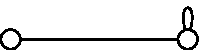
\includegraphics{diagrams/self-loops}\\
  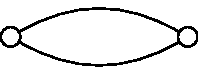
\includegraphics{diagrams/multiple-edges}\\
  
\includegraphics{diagrams/directed-graph}
  \caption{Self loops, duplicate edges and arrows are not allowed.}
  \label{fig:bad-graphs}
\end{figure}

A \textbf{directed graph} is just like a normal graph, except the edges do have
arrows. The only mathematical difference is that the set $E$ is a set of ordered
pairs.

The \textit{degree} of a node in a graph, is the number of edges that are
adjacent to (touching) it. If the graph is directed, then it is the number of
edges originating from the node.

A weighted graph is one where each edge is associated with a value representing
its weight. The length of a path between nodes is simply the sum of the edge
weights connecting the nodes.

\subsection{Connectivity}
\label{connectivity}

A node $a$ is \textbf{reachable} from another node $b$ if there is some sequence
of nodes connected by edges that go from the $a$ to $b$.

A graph where every node is reachable from every other node is
\textbf{connected}. A strongly connected graph is a \textbf{directed graph}
where each node is reachable from each other node.

\begin{figure}[h]
  \centering
  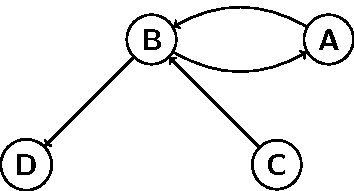
\includegraphics{diagrams/connected-graph}
  \caption{This graph is not strongly connected, but the subgraph with only
  nodes $A$ and $B$ is. If we were to remove the arrows, then the graph would
  be connected.}
  \label{fig:connected-graph}
\end{figure}

\subsection{Representing graphs}

We can store graphs in computer memory in two ways:

\begin{description}
  \item \textbf{Adjacency List}\\
    There are two different kinds of adjacency list, the first is like so:

    \begin{lstlisting}[language=java]
      public class Graph {
        List<Vertex> nodes;
        List<Edge> edges;
      }
      public class Edge { Vertex a, b; }
      public class Vertex { List<Edge> outlist; }
    \end{lstlisting}

    Here, we keep a list of all the nodes, and a list of all the edges. From
    any edge, we can see what nodes it connects, and from any node, we can
    see what edges it connects.

    The other type of adjacency list is a bit simpler, but less efficient in
    some cases:

    \begin{lstlisting}[language=java]
      public class Graph<T> {
        Set<T, List<T>> adjList;
      }
    \end{lstlisting}
  \item \textbf{Adjacency Matrix}\\
    Here, a matrix indicates whether there is an edge between two nodes:

    \begin{center}
      \begin{tabular}{c|c c c c}
          & A & B & C & D\\ \hline
        A & 0 & 1 & 0 & 0\\
        B & 1 & 0 & 0 & 1\\
        C & 0 & 1 & 0 & 0\\
        D & 0 & 0 & 0 & 0\\
      \end{tabular}
    \end{center}

    This adjacency matrix represents the graph in
    Figure~\ref{fig:connected-graph}. You can see that it is fairly wasteful
    in terms of memory $O(|E|* |V|)$, though with bit arrays, it has a very 
    low constant overhead.
\end{description}

\subsection{Classifying Edges}

During a \textit{depth first traversal} (Section~\ref{depth-first-search}) of a
graph, we can classify each edge into one of four types. When doing the
traversal, we process each edge from left to right (from the viewer's
perspective), and we define an edge to be an \textit{ancestor} of another edge
if there is a path from the ancestor edge to the descendent edge and the ancestor
is traversed first. The four types of edges are:

\begin{description}
  \item \textbf{Tree edges}\\
    These edges lead to a new node during a search. If you remove all the edges 
    from the graph except tree edges, then you get a tree!
  \item \textbf{Forward edges}\\
    These go from ancestor edges to descendent edges, but are not tree edges
    (i.e. the descendent node has been visited already).
  \item \textbf{Cross edges}\\
    These go between edges where no node is the ancestor of the other.
  \item \textbf{Back edges}\\
    An edge that goes from a descendant to an ancestor.
\end{description}

\begin{figure}[h]
  \centering
  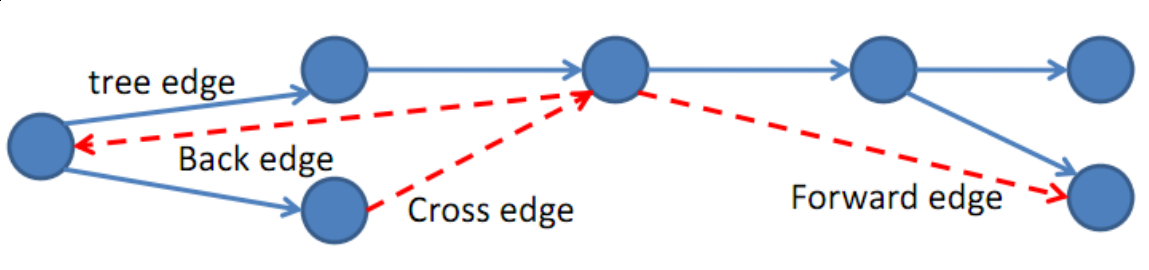
\includegraphics[width=0.6\textwidth]{images/edge-types}
  \caption{A
  \href{http://courses.csail.mit.edu/6.006/spring11/rec/rec13.pdf}{pictorial
  illustration} of the different edge types.}
  \label{fig:connected-graph}
\end{figure}

\subsection{Graph Algorithms}

You will have covered some of the algorithms featuring here in previous courses,
or perhaps seen them in the wild. They are however interesting and useful, so
it's worth a recap even if they're not new! I've ordered these in roughly
increasing order of mental strain.

\subsubsection{Depth first search}
\label{depth-first-search}

\href{https://en.wikipedia.org/wiki/Depth-first_search}{Depth first search}
(DFS) is an algorithm to find a node in a graph starting from another node. It
works on both directed and undirected graphs, and runs in $O(|V| + |E|)$
(linear) time. The psudo code looks like this:

\marginpar{Note how we mark nodes as having been visited (by adding them to
\texttt{visitedNodes}). This is so if there is a loop in the graph, the 
algorithm doesn't run indefinitely.}

\begin{lstlisting}[language=java]
  Node dfs(Node haystack, Node needle) {
    Stack<Node> toVisit = new Stack<>();
    Set<Node> visitedNodes = new Set<>();
    toVisit.push(haystack);
    while(!toVisit.isEmpty()) {
      Node node = toVisit.pop();
      if (visitedNodes.contains(node)) continue;
      visitedNodes.add(node);
      if(node.equals(needle)) {
        return needle;
      } else {
        for(Node child : node.children) {
          toVisit.push(child);
        }
      }
    }
    return null;
  }
\end{lstlisting}

A Breadth First Search is the same, except you use a \texttt{Queue} instead of a
\texttt{Stack}.

\marginpar{To see if a graph is connected, do a depth first search as in the
example code, but don't stop when you find a needle, only stop when the
\texttt{toVisit} stack is empty. If \texttt{visitedNodes} contains all of the
nodes in the graph, then the graph is connected.}

Depth first search also lets you find if one node is reachable from another in
linear time, and also if a graph is connected in linear time too, with a few
modifications.

We can also find out if a directed graph is strongly connected in $O(|V| + |E|)$
time using Tarjan's algorithm, which we'll see later.

\subsubsection{Dijkstra's algorithm}

Dijkstra's algorithm finds the undirected shortest path between two nodes in a
graph. Here is the psudo-code:

\marginpar{My best advice for learning an algorithm like this, is to get a 
whiteboard, draw out the problem, and then run the solution manually on the 
whiteboard. Then you have a pictorial and visual explanation of how the 
algorithm \textit{really} works.}

\begin{lstlisting}[language=java,
                  caption=Dijkstra's algorithm (from Wikipedia),
                  label=lst:dijkstra,
                  captionpos=b]
function Dijkstra(Graph, source):
  create vertex set Q

  // Initialization
  for each vertex v in Graph:
    dist[v] = INFINITY
    prev[v] = UNDEFINED
    add v to Q

  // Distance from source to source
  dist[source] = 0

  while Q is not empty:
    u = vertex in Q with min dist[u]
    remove u from Q 

  for each neighbour v of u:
    alt = dist[u] + length(u, v)
    // A shorter path to v has been found
    if alt < dist[v]:
      dist[v] = alt 
      prev[v] = u 

  return dist[], prev[]
\end{lstlisting}

If we use a Fibonacci heap, for the priority queue, then the runtime of
Dijkstra's algorithm is $O(|E| + |V|log(|V|)$. If we use a normal heap, then the
runtime is $O(|E|log(|V|))$.

\subsubsection{Tarjan's Algorithm}

Before we delve into Tarjan's Algorithm, we need to discuss strongly connected
components. You will remember from Section~\ref{connectivity}, that a graph is
strongly connected if all nodes are reachable from any other node.

A \textit{strongly connected component} is a subset of edges within a graph,
where the subset is strongly connected. If a graph has only one strongly
connected component, then it is strongly connected.

The psudo code here is from
\href{https://en.wikipedia.org/wiki/Tarjan%27s_strongly_connected_components_algorithm}{Wikipedia}.
If you're reading this after week 8 of the \texttt{COMP36111} course, then you
probably have your own implementation in C.

\begin{lstlisting}
  algorithm tarjan is
  input: graph G = (V, E)
  output: set of strongly connected components (sets of vertices)

  index := 0
  S := empty
  for each v in V do
    if (v.index is undefined) then
      strongconnect(v)
    end if
  end for

  function strongconnect(v)
    // Set the depth index for v to the smallest unused index
    v.index := index
    v.lowlink := index
    index := index + 1
    S.push(v)
    v.onStack := true

    // Consider successors of v
    for each (v, w) in E do
      if (w.index is undefined) then
        // Successor w has not yet been visited; recurse on it
        strongconnect(w)
        v.lowlink  := min(v.lowlink, w.lowlink)
      else if (w.onStack) then
        // Successor w is in stack S and hence in the current SCC
        v.lowlink  := min(v.lowlink, w.index)
      end if
    end for

    // If v is a root node, pop the stack and generate an SCC
    if (v.lowlink = v.index) then
      start a new strongly connected component
      repeat
        w := S.pop()
        w.onStack := false
        add w to current strongly connected component
      while (w != v)
      output the current strongly connected component
    end if
  end function
\end{lstlisting}

%TODO: Expand on Tarjan's algorithm when a whiteboard is present

\section{Linear Programming}

Linear programming is an optimisation problem, where we want to find the `best'
solution to a set of equations. We're going to solve it using the
\textit{simplex} method, but before we do, I think it's a good idea to recap
some high-school mathematics first. Feel free to skip the next subsection if
you're feeling confident with it.

\subsection{Background mathematics}

An inequality relation is just like a normal equation, except the equals sign is
replaced by either $<$, $>$, $\leq$ or $\geq$. When you solve an inequality, you
generally want to get all of the similar terms on one side (e.g. move all the
variable terms over to one side, and all of the constants to another side). This
\textit{mostly} works like a normal equation; you can add and subtract from both
sides just like normal, however, if you want to divide or multiply \textbf{by a
negative quantity}, then you need to \textbf{reverse the equality}.

\[
  \begin{split}
    -2x &> -2\\
    2x &< 2\\
    x &< 1
  \end{split}
\]

This equality is satisfied whenever $x$ is less than $1$. If we have two terms
in the equality (something similar to $ax + by \geq c$), it becomes slightly
harder to solve. To solve this we can:

\begin{itemize}
  \item Plot a graph of the line $ax + by = c$.
  \item Pick a test point $(x, y)$ not on the line, and plot it on the graph.
  \item If the point $(x, y)$ satisfies the inequality, then shade the opposite 
    side of the line to which the point is on, otherwise, shade the same side.
\end{itemize}

For example, given $3x + 4y \leq 6$, and choosing the point $(-2,1)$ we end up
with what's in Figure~\ref{fig:graph-1}.

\begin{figure}[h]
  \centering
  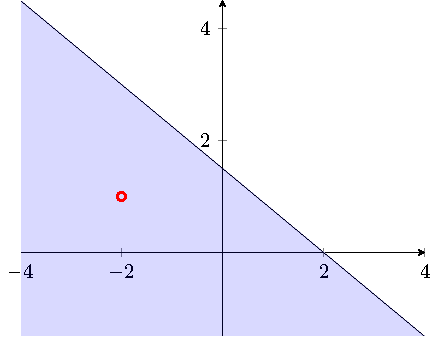
\includegraphics{diagrams/graph1}
  \caption{A graph of $3x + 4y \leq 6$, with all the valid values shaded blue.}
  \label{fig:graph-1}
\end{figure}

If we have multiple inequalities, we want to \textit{find the region where all
of them are satisfied}. This involves plotting each line, and shading the
regions where they're not satisfied, which means the blank bit is the bit we
want.

If we have the equations $3x + 4y \leq 6$, $2y - x \leq 2$ and $x \geq 0$, we
will get something like in Figure~\ref{fig:graph-2}.

\begin{figure}[h]
\captionsetup{width=.4\linewidth}
\centering
\begin{minipage}{.5\textwidth}
  \centering
  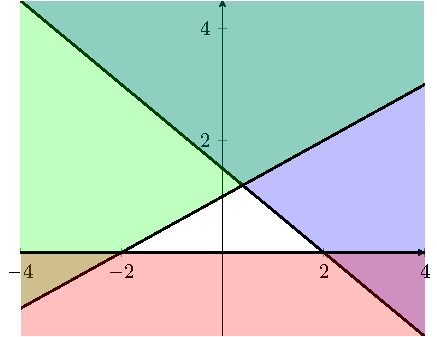
\includegraphics[width=\textwidth]{diagrams/graph2}
  \captionof{figure}{A graph plotting $3x + 4y \leq 6$, $2y - x \leq 2$ and
  $x \geq 0$, where the points not satisfying the inequalities are shaded in 
  blue, green and red respectively. The clear region satisfies all points.}
  \label{fig:graph-2}
\end{minipage}%
\begin{minipage}{.5\textwidth}
  \centering
  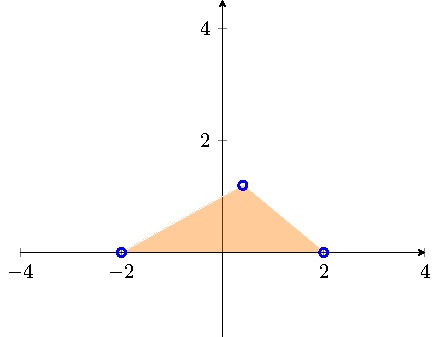
\includegraphics[width=\textwidth]{diagrams/graph3}
  \captionof{figure}{The valid region in the three inequalities from
  Figure~\ref{fig:graph-2}. The corner points are $(2,0),(-2,0)$ and
  $(\frac{2}{5},\frac{6}{5})$.}
  \label{fig:graph-3}
\end{minipage}
\end{figure}


The corner points are especially important to us, since that's often where the
useful numbers are (we'll see more of this later). In order to find the corner
points, we solve the two lines that form them. Solving the following equations
gives the points in Figure~\ref{fig:graph-3}.

\begin{mymulticols}
  \begin{itemize}
    \item $x = 0, 3x + 4y = 6$
    \item $x = 0, 2y - x = 2$
    \item $2y - x = 2, 3x + 4y = 6$
  \end{itemize}
\end{mymulticols}

So, now we know how to solve these types of problems, lets look at how to
decompose a problem statement into a set of equations.

\begin{quote}

  You can buy wood in 11 meter lengths, or 6 meter lengths. A 11 meter piece of
  wood can be cut into two lengths of 5 meters, and one length of 1 meter. A 6
  meter piece of wood is cut into one length of 5 meter, and one length of 1
  meter.

  If we have room for twenty 1 meter pieces and thirty 5 meter pieces, how many
  11, and how many 6 meter lengths should we buy? We cannot go over that amount
  of pieces, but we can settle for less than that amount.

\end{quote}

To answer this, we can make a table to describe it:

\begin{center}
  \begin{tabular} {|p{3cm}|p{2cm}|p{2cm}|}
    \hline
    \multirow{2}{*}{Bought Length} & \multicolumn{2}{c|}{Required length}\\
    \cline{2-3}
    & 5 meter & 1 meter\\ \hline
    11 meter\newline 6 meter & 2 per board\newline 1 per board & 1 per
    board\newline 1 per board\\ \hline
    Amount needed & 30 & 20\\ \hline
  \end{tabular}
\end{center}

This decomposes into the following equations:

\begin{itemize}
  \item $2x + y \leq 30$
  \item $x + y \leq 20$
  \item $x \geq 0$, $y \geq 0$
\end{itemize}

\marginpar{Notice how our shapes always have a convex hull...}

Plotting this on a graph gives us what's in Figure~\ref{fig:graph-4}, where we
can see a feasible region between $(0, 20), (10, 10), (15, 0)$ and  $(0,0)$. The
three corner points are all of the non-zero points (zero eleven meter and zero
six meter pieces is an invalid solution), and anywhere on the outer edge of the
region is a solution.

\begin{figure}[h]
  \centering
  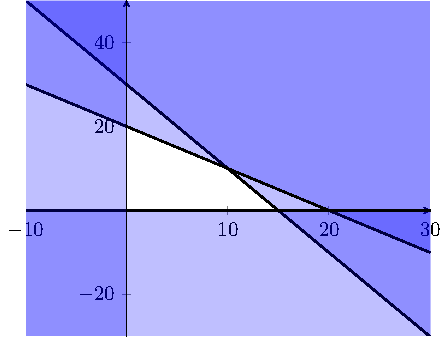
\includegraphics{diagrams/graph4}
  \caption{A graph of $2x + y = 30$, $x + y = 20$, $x > 0$, $y > 0$.}
  \label{fig:graph-4}
\end{figure}

\subsection{The maximum problem}

Sometimes, we want to maximise some particular variable. For example, companies
want to maximise their profit. If this is the case, then we can come up with a
function for the profit, something like:

\[
  P = 7x + 3y
\]

Where $x$ is the number of $5$ meter boards, and $y$ is the number of $1$ meter
boards. We can factor this equation into our solution, to find the most
profitable wood to buy.

If you think about it, the further from the origin we get, the more profit we
get. At $(0,0)$ we have no profit, since we have done nothing, but at $(5,0)$ we
have $35$ profit since we have bought five, $5$ meter length boards. Since our
lines always intersect to produce a region with a convex shape, the points
furthest from the origin are the corner points. To figure out how much profit we
can make, we just need to find the maximum of these points:

\begin{center}
  \begin{tabular}{c | c | c | c}
    \textbf{Corner point} & \textbf{5 meter boards} & \textbf{1 meter boards}
      & \textbf{Profit}\\  \hline
    $(0,20)$  & 20 & 20 & 200\\ \hline
    $(10,10)$ & 30 & 20 & 270\\ \hline
    $(15,0)$  & 30 & 15 & 255\\
  \end{tabular}
\end{center}

Therefore the most profitable choice is to buy $10$ 11 meter length boards and
$10$ 6 meter length boards.

\subsection{The Simplex Method}

If we have more than two variables, then all of a sudden, working out the
optimum on a graph becomes rather hard. Drawing 3d graphs is hard, and
visualising n-dimensional graphs quickly becomes infeasible.

The simplex method automates finding the optimum value of any number of
variables. This is how it works:

\begin{itemize}
  \item Draw the feasible region in $n$ dimensional space
  \item Select a corner of the feasible region
  \item Choose an edge that is connected to this point that will increase the
  objective function.
  \item Go to the next corner on that edge
  \item Keep doing steps 3 and 4 until you find an optimal solution.
\end{itemize}

That's pretty far removed from how we see the simplex algorithm working, since
we find the optimum by using a tableaux. I've broken down the algorithm into
multiple steps with a running example here:

\begin{itemize}
  \item[\textbf{Step 0}] The zero'th step, is to examine the input data we're 
  given. This will consist of a function $f$ to be maximised and a set of 
  inequalities that constrain the values we can give to $f$.

  \[\begin{split}
    f &= 10x + 12y +12z\\
    3 &\geq 5x + 2y + z\\
    2&\geq x + 2y + 4z\\
  \end{split}\]

  N.b. if the inequalities aren't of the form $CONST \geq EXPR$, then rearrange 
  them so that they are.

  \item[\textbf{Step 1}] Now we turn each inequality we were given into an 
  equation (replace the inequality sign with an equals basically), and introduce 
  a new variable for each (called a \textit{slack variable}). Also, rearrange
  $f$ so its equal to zero:

  \begin{alignat*}{12}
    3 &=~ &5x~  &+~&2y~ &+~&z ~&+~&m_1&~ &~  &~ &~  &~&~\\
    2 &=~ &~x   &+~&2y~ &+~& z~&~~&~  &+~&m_2&~ &~  &~&~\\
    0 &=~ &-10x~&-~&12y~&-~&12z&~ &~  &~ &~  &~ &~  &+&f
  \end{alignat*}
  \item[\textbf{Step 2}] Now our problem is in the correct form, we can whack it 
  into a tableaux:

  \begin{center}
    \begin{tabular}{>{$}c<{$}|>{$}c<{$}|>{$}c<{$}|>{$}c<{$}|>{$}c<{$}|
      >{$}c<{$}|>{$}c<{$}|>{$}c<{$}|>{$}c<{$}}
          & x & y & z & m_1 & m_2 & m_3 & f & \text{constants}\\ \hline
      m_1 & 5 & 2 & 1 & 1   & 0   & 0   & 0   & 3\\ \hline
      m_2 & 1 & 2 & 4 & 0   & 1   & 0   & 0   & 2\\ \hline
      f   &-10&-12&-12& 0   & 0   & 0   & 1   & 0\\
    \end{tabular}
  \end{center}

  It should be quite obvious how we go from the equations in step 1 to the
  tableaux in here. The only stuff you need to \textit{remember} about
  formatting the tableaux, is that the slack variables go along the left side,
  $f$ is the bottom row, and to put the constants in the last column.

  The values in the bottom row are called \textbf{indicators}.

  \item[\textbf{Step 3}] We need to find the \textbf{pivot cell} in the table. 
  The pivot column is easy to find, its the one with the most negative 
  indicator (in our case, the second or third column, since the indicators 
  there are $-12$, we're picking column two for no particular reason). 
  Finding the row is a bit harder, you need to divide the constant column by 
  the pivot column and pick the one with the lowest value:

  \marginpar{\textbf{Only choose positive ratios}, and remember that
  $?/0 = \infty$. Otherwise it goes belly up and it takes you over a day to 
  figure out why (this may or may not have  happened to me...).}

  \definecolor{highlight}{gray}{0.7}
  \definecolor{dhighlight}{gray}{0.5}

  \begin{center}
    \begin{tabular}{>{$}c<{$}|>{$}c<{$}|
      >{$}>{\columncolor{highlight}}c<{$}|>{$}c<{$}|>{$}c<{$}|
      >{$}c<{$}|>{$}c<{$}|>{$}c<{$}|>{$}c<{$}|c}
          & x & y & z & m_1 & m_2 & m_3 & f & \text{constants}
            & \text{ratio}\\ \hline
      m_1 & 5 & 2                       & 1 &1& 0& 0&0&3 & 3/2 \\ \hline
      \rowcolor{highlight}
      m_2 & 1 &\cellcolor{dhighlight} 2 & 4 &0& 1& 0&0&2 & 2/2\\ \hline
      f   &-10&-12                      &-12&0& 0& 0&1&0 & N/A \\
    \end{tabular}
  \end{center}

  \item[\textbf{Step 4}] Now we do the pivot about the pivot cell:

    \begin{itemize}
      \item[\textbf{Step 4a}] Divide each cell in the pivot's row by the pivot
      (which makes the pivot equal to $1$!).

      \begin{center}
        \renewcommand{\arraystretch}{1.2}
        \begin{tabular}{>{$}c<{$}|>{$}c<{$}|
          >{$}c<{$}|>{$}c<{$}|>{$}c<{$}|
          >{$}c<{$}|>{$}c<{$}|>{$}c<{$}|>{$}c<{$}}
              & x & y & z & m_1 & m_2 & m_3 & f & \text{constants}\\ \hline
          m_1 & 5 & 2 & 1 &1& 0& 0&0&3\\ \hline
          \rowcolor{highlight}
          m_2&\frac{1}{2}&\cellcolor{dhighlight}1&2&0&\frac{1}{2}&0&0&1\\ \hline
          f   &-10&-12&-12&0& 0& 0&1&0\\
        \end{tabular}
      \end{center}

      \item[\textbf{Step 4b}] Subtract the pivot row from each other row
      so that the whole pivot column becomes $0$. For example here, we need to
      $R1 = R1 - 2(R2), R3 = R3 + 12(R2)$ to make the cell below 
      the pivot $0$.

      \begin{center}
        \renewcommand{\arraystretch}{1.2}
        \begin{tabular}{>{$}c<{$}|>{$}c<{$}|
          >{$}c<{$}|>{$}c<{$}|>{$}c<{$}|
          >{$}c<{$}|>{$}c<{$}|>{$}c<{$}|>{$}c<{$}}
              & x & y & z & m_1 & m_2 & m_3 & f & \text{constants}\\ \hline
          m_1 & 4 & 0 &-3 &1&-1& 0&0&1\\ \hline
          m_2 & \frac{1}{2} & 1& 2 &0&\frac{1}{2}&0&0&1\\ \hline
          f   &-4 & 0 & 12&0& 6& 0&1&12\\
        \end{tabular}
      \end{center}

      \item[\textbf{Step 4c}] Replace the letter on the pivot row with the 
      letter on the pivot column:

      \begin{center}
        \renewcommand{\arraystretch}{1.2}
        \begin{tabular}{>{$}c<{$}|>{$}c<{$}|
          >{$}c<{$}|>{$}c<{$}|>{$}c<{$}|
          >{$}c<{$}|>{$}c<{$}|>{$}c<{$}|>{$}c<{$}}
              & x & y & z & m_1 & m_2 & m_3 & f & \text{constants}\\ \hline
          m_1 & 4 & 0 &-3 &1&-1& 0&0&1\\ \hline
          y & \frac{1}{2} & 1& 2 &0&\frac{1}{2}&0&0&1\\ \hline
          f   &-4 & 0 & 12&0& 6& 0&1&12\\
        \end{tabular}
      \end{center}
    \end{itemize}

    \item[\textbf{Step 5}] Now we have found another solution, to see what it 
    is, read off the letters on the far left and correspond them to the 
    constants on the far right:

    \[
      x = 0, y = 1, z = 0, m_1 = 1, m_2 = 0, f = 12
    \]

    If we sub that in, then we can see that if satisfies the formulae from step
    1:

    \begin{alignat*}{12}
      3 &=~ & 0~  &+~&2~ &+~&0 ~&+~&  1&~ &~  &~ &~  &~&~\\
      2 &=~ &~0   &+~&2~ &+~&0 ~&~~&~  &+~&  0&~ &~  &~&~\\
      0 &=~ &-0  ~&-~&12~&-~&0  &~ &~  &~ &~  &~ &~  &+&12
    \end{alignat*}

  \item[\textbf{Step 6}] If there are no negative indicators in the table
  (bottom row of the tableaux), then we've finished, and our solution is the 
  optimal one. If there are, then we need to go back to step 3 and repeat until 
  there aren't any negative indicators. Since we have a negative indicator in 
  the first column, then we should loop back and do another iteration.

\end{itemize}

If we run steps 3-6 again (which we should do because there is a
negative indicator), we get the optimum, which is:

\begin{center}
  \renewcommand{\arraystretch}{1.2}
  \begin{tabular}{>{$}c<{$}|>{$}c<{$}|
    >{$}c<{$}|>{$}c<{$}|>{$}c<{$}|
    >{$}c<{$}|>{$}c<{$}|>{$}c<{$}|>{$}c<{$}}
        & x & y & z & m_1 & m_2 & m_3 & f & \text{constants}\\ \hline
    x & 1 & 0 &\frac{-3}{4}&\frac{1}{4} &\frac{-1}{4}&0&0&\frac{1}{4}\\ \hline
    y & 0 & 1 &\frac{19}{8}&\frac{-1}{8}&\frac{5}{8} &0&0&\frac{7}{8}\\ \hline
    f & 0 & 0 & 9          & 1          & 5          &0&0&13\\
  \end{tabular}
\end{center}

So:

\[
  f = 13,~x = 0.25,~y = 0.825,~z = 0
\]

You can use this tool to check solutions to simplex problems:
\url{http://www.zweigmedia.com/RealWorld/simplex.html}.

\subsubsection{Duality}

Simplex is great if we're trying to maximise a function, but what if we want to
minimise it? Duality does this. Basically, you give it a function and
inequalities, it mutates them so they'll fit into simplex, and then you run
simplex as normal. So, to apply the duality theorem, you need:

\begin{itemize}
  \item A function you want to minimize; $f = ax + by + \dots$
  \item A set of inequalities of the form `$EXPR \geq CONST$'
\end{itemize}

Since simplex tries to maximise $f$, which is the opposite of what we want to
do, and our inequalities are the wrong way around, we need to the duality bit
now:

First, like the first part of simplex, we put the coefficients in a table.
However, this table has a special name; the \textit{coefficient matrix}. It's
called a matrix, not a table because we're going to do a transposition on it
(and mathematicians transpose matrices, not tables!). 

The input:

\[
  \begin{split}
    g = 3r + 4s + t\\
    r + 2s + t \geq 4\\
    r + 2s - t \geq -2\\
    r + s \geq -1\\
    r \geq 0,~s \geq 0,~t \geq 0
  \end{split}
\]

Would result in a matrix like this:

\begin{center}
  \begin{tabular}{>{$}r<{$}|>{$}c<{$} >{$}c<{$} >{$}c<{$} >{$}l<{$}}
        & r & s & t & \text{constants}\\ \hline
        & 1 & 2 & 1 &4\\ 
        & 1 & 2 &-1 &-2\\ 
        & 1 & 1 & 0 &-1\\ 
      g & 3 & 4 & 1 &  \\ 
  \end{tabular}
\end{center}

So, we put the inequalities in first, then put the minimising function in the
last column. Now what we do, is to flip the matrix along its top-left to bottom-
right diagonal:

\begin{center}
  \begin{tabular}{>{$}r<{$}|>{$}c<{$} >{$}c<{$} >{$}c<{$} >{$}l<{$}}
        & x & y & z & \text{constants}\\ \hline
        & 1 & 1 & 1 & 3\\ 
        & 2 & 2 & 1 & 4\\ 
        & 1 &-1 & 0 & 1\\ 
      f & 4 &-2 &-1 &  \\ 
  \end{tabular}
\end{center}

After we've done that, we get the following equation and inequalities:

\[
  \begin{split}
    f = 4x - 2y - z\\
    x + y + z \leq 3\\
    2x + 2y + z \leq 4\\
    x + y \geq 1\\
    x \geq 0, y \geq 0,~z \geq 0
  \end{split}
\]

If you do simplex on them (you should try it for practice!), you get:

\begin{center}
  \renewcommand{\arraystretch}{1.2}
  \begin{tabular}{>{$}c<{$}|>{$}c<{$}|
    >{$}c<{$}|>{$}c<{$}|>{$}c<{$}|
    >{$}c<{$}|>{$}c<{$}|>{$}c<{$}|>{$}c<{$}l}
        & x & y & z & m_1 & m_2 & m_3 & f & \text{constants}\\
    \cline{1-9}
    w_1& 0 & 0 &\frac{1}{2}& 1 &\frac{-1}{2}&0&0&1&\\
    \cline{1-9}
    y & 0 & 1 &\frac{1}{4}&0&\frac{1}{4} &\frac{-1}{2}&0&\frac{1}{2}&\\
    \cline{1-9}
    x & 1 & 0 &\frac{1}{4}&0&\frac{1}{4}&\frac{1}{2}&0&\frac{3}{2}&\\
    \cline{1-9}
    f & 0 & 0 &\frac{3}{2} & 0 & \frac{1}{2}   &3&1&5&g\\
    \multicolumn{4}{c}{~}&\multicolumn{1}{c}{r}&\multicolumn{1}{c}{s}&
    \multicolumn{1}{c}{t}&\multicolumn{2}{c}{~}
  \end{tabular}
\end{center}

Therefore the minimum value of $g$ is $5$, with the inputs as $r=0$,
$s=\frac{1}{2}$, $t=3$.

The course reading, sums up the duality theorem like so (in your head, replace
`dual problem' with `simplex problem'):

\begin{quote}
  The minimum value of the objective function $g = ar + bs + ct$ in a primal
  minimization problem is the maximum value of the objective function $f = ax +
  by + cz$ in the dual problem. Values of $r,~s$ and $t$ that minimize $g$
  appear in the lat row of the terminal tableau of the dual problem under the
  slack variables $w_1,~w_2$ and $w_3$.
\end{quote}

\subsubsection{Complexity}

The Simplex algorithm has an exponential complexity, since in the worst case,
adding a new inequality results in having twice as many vertices to traverse as
before.

An interesting aspect of the Simplex algorithm, is that although there are
polynomial alternatives, in practice it beats all the other algorithms! Is this
because we only ever run it on the inputs which are solvable in polynomial time?

\section{Integer Programming}

Integer programming is just like linear programming, except we are only allowed
solutions inside $\mathbb{N}$ (the integers) instead of $\mathbb{R}$ (real
numbers). Even though we've narrowed our search space, the new problem turns out
to be harder (remember, even though our solutions will be finite and countable,
there are still a lot (very exponential) of them)!

We define \textit{mixed integer programming} to be linear programming, where
some variables are integers, but some are real numbers. Likewise, \textit{pure
integer programming} is when all the variables are integers.

At first, I thought integer programming was a bit pointless; couldn't you just
find the linear programming solution, and then round it down to the nearest
integer? Well, yes, but there are two issues; firstly, it might not be the best
solution, and secondly, you can do cool stuff with integer programming.

For example, what if we wanted to implement multiple choice? Say I want to buy
either car A, B, or C, and they all have safety ratings, prices, etc. I
obviously can't buy 0.375A, 0.005B and 0.62C; I have to make a decision.

We can encapsulate this in integer programming by having a constraint like this:

\[
  A + B + C \leq 1
\]

Furthermore, we can restrict variables to be binary too, which, if all our
variables are binary, actually turns out to be our old friend the knapsack
problem!

In fact, any pure integer programming problem can be expressed as a 0-1 problem,
since we can express any decimal number as a binary number.

\marginpar{We can also turn scheduling problems such as timetabling or the 
travelling salesman problem into integer programming problems.}

You may have worked out by this (if you remember the lectures from the second
half of this course, or if you have read later sections of this document), that
if we can turn the 0-1 knapsack problem into an integer programming problem,
then integer programming must be in the same complexity class as the knapsack
problem; meaning that integer programming is NP hard!

\subsection{Solving Integer Programming Problems}

It turns out, that \textit{Branch and Bound} is a good way to solve these kinds
of problems. If you remember the second year algorithms course, then you might
be having a quiet little groan right now. However, I have good news! There's a
really good explanation of B\&B in the course reading (The Chapter 9 handout you
should have picked up in the lecture).

Though it's good, and thorough, it's also a bit boring and dense. Here's my
shorter version, broken up into steps:

\begin{enumerate}
  \item So, we have an optimisation problem just like normal. We can graph it, 
  and it'll look something like this:

  \begin{figure}[H]
    \centering
    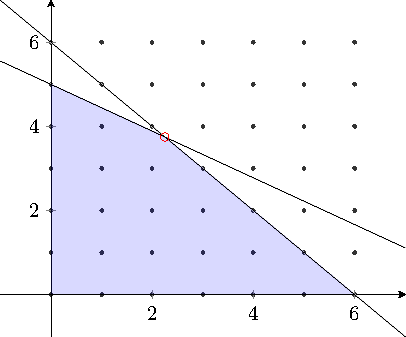
\includegraphics{diagrams/graph5}
    \caption{A graph of $y = 6 - x$, $y = \frac{45 - 5x}{9}$ and $x \geq 0,
      y \geq 0$. The linear optimum is shown as the red circle.}
    \label{fig:graph-5}
  \end{figure}

  This of course is a graph of two constraints relating to a maximisation
  problem. The problem and constraints are here:

  \[
    \begin{split}
      f = 5x + 8y\\
      x + y \leq 6\\
      5x + 9y \leq 45
    \end{split}
  \]

  If we use Simplex to solve this like a linear programming problem, then we get
  the optimum as $f(\frac{9}{4}, \frac{15}{4}) = 41.25$, which is obviously not
  a integral solution (since it has fractions).

  One thing to do might be to round off the numbers, trying $(2,4)$, which is
  infeasible due to the constraints and $2,3$ which gives $f=34$. However, while
  the latter solution is feasible, it is \textit{not} the optimum.

  \textbf{Note, in an example like this, you could enumerate all the integral 
  points and find which one is best. This was mentioned in the lectures and is 
  a lot easier than doing Branch and Bound!}

  \item If we don't have time to enumerate the points, then we need to do 
  branch and bound. We make use of the following observations:
  
  \begin{itemize}
    \item The integral solution isn't the same as the linear one for this
      problem, since the linear solution is not integral.
    \item The linear solution provides an upper bound on the integral solution.
  \end{itemize}

  In order to progress, you split the feasible region into half, along where
  either the $x$ or $y$ axis is equal to the linear optimum. We could split at
  $x = \frac{9}{4}$ or $y = {15}{4}$, and will do the latter. Since our
  solutions are integral, we can discard the area between $3 < y < 4$:

  \begin{figure}[H]
    \centering
    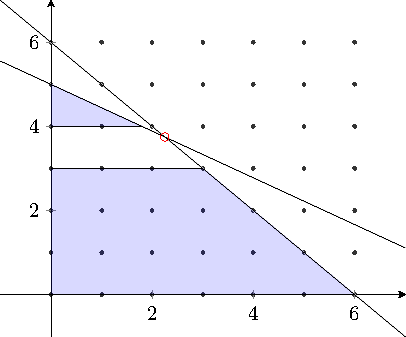
\includegraphics{diagrams/graph6}
    \caption{Now, we're showing the two feasible regions after we've split 
      along $y = \frac{15}{4}$}
    \label{fig:graph-6}
  \end{figure}

  Now, we have two problems; finding the integral solution to the upper region,
  and the lower region. Then we can simply pick the maximum!

\item To find the integral solution to each sub-region, simply add a new 
  constraint for each; for the top one, we add $y \geq 4$, and for the bottom 
  one, we add $y \leq 3$. Then we recurse to step 1 on both problems.

  However, because I'm nice, I'm going to do the recursion for you here:

  \begin{description}

  \item \textit{Top recursion}\\
  If we do this, we find that the linear solution for the top problem is
  $(\frac{9}{5}, 4)$, where $f = 41$. This isn't an integral, but we have gained
  important information; we can split the top area into two:

  \begin{figure}[H]
    \centering
    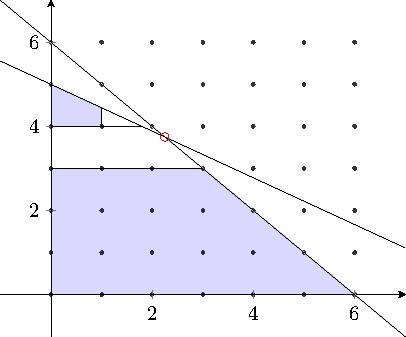
\includegraphics{diagrams/graph7}
    \caption{I've split the top area into two new areas where $x \leq 1$ and
    $x \geq 2$. Ohh wait, there aren't any integral points inside that last 
    one, so it's not shaded :)}
    \label{fig:graph-7}
  \end{figure}

  If we recurse again, we will find that the top part \textit{still} doesn't
  have an integral solution, but another level of recursion gives us two
  integral solutions (this is obvious if you think about it, since we can't
  recurse any more times due to the number of possible integer points inside the
  region); $f(1,4) = 37$, and $f(0,5) = 40$.

  \item \textit{Bottom recursion}\\
  If we recurse on the bottom region, and to simplex on it, we get an integral
  solution straight away; $f(3,3) = 39$. Since we know that the linear solution
  is an upper bound on the integral solution (hence we won't find a larger
  answer inside the rest of the lower region), then we can stop here.
  \end{description}

  Since the top region's result $f(0,5) = 40$ was better than the bottom
  region's one $f(3,3) = 39$, and those regions had inside them all the
  feasible points, then we have found our solution, $f(0,5) = 40$.

  If you understood all that, then I recommend you read Chapter 9 of the course
  handout (from section 9.4 on page 287 to the end of section 9.5 on page 292),
  since it visualises the above as a tree as well. Besides, you've already
  understood the concept, so it'll be light reading!

\end{enumerate}

\section{Flow Matching}

Like integer programming, flow matching is a problem that initially seems quite
niche, but actually has a lot of applications. In essence, given a weighted
graph, a `start' node and an `end' node, we want to compute the \textit{maximum
flow} through the graph from the source to the target. Imagine each edge is a
pipe between nodes, and liquid flows through the pipe. The weight of each edge
indicates how much liquid can flow through the graph, and a flow defines how
much liquid is flowing through each edge.

While flow matching, at first glance, seems only applicable to things like oil
pipelines and plumbing, we can actually map lots of problems onto graphs and
weighted edges.

\subsection{The stable marriage problem}

Given $n$ boys and $n$ girls, and a list for each boy and each girl of who they
would marry (this is binary; a yes/no thing), we want to come up with a $1-1$
pairing between the boys and the girls that produces the maximum number of
couples.

If we define that mathematically, then we let $G = (V, W, E)$, where $G$ is a
bipartite graph\marginpar{A bipartite graph is one who's nodes can be divided
into two disjoint sets, such that every edge in one of the sets connects to one
in the other.}, $V$ is the set of boys, $W$ is the set of girls and $E$ is the
set of edges. An edge from $v$to $w$ indicates that $v$ and $w$ both would marry
eachother.

$E' \subset E$ such that for all $v \in V$, there is at most one $w \in W$, and
for all $w \in W$, there is at most one $v \in V$. I.e, $E'$ is a matching
between the boys and girls, which is a subset of their preferences for each
other.

If every node has one edge (each item in $V$ and $W$ is incident to some $e \in
E'$), then the matching is perfect.

We can define the stable marriage problem to return \texttt{yes} if the input
graph has a perfect matching, and \texttt{no} otherwise.

A naive way of solving the problem is to iterate over each possible matching and
see if it is perfect:

\begin{lstlisting}[language=Java]
  boolean naiveSoln(ImmutableSet<Node> boys, ImmutableSet<Node> girls,
      ImmutableSet<Edge> preferences) {
    if (boys.isEmpty()) {
      return girls.isEmpty();
    } else {
      Node randomBoy = boys.getRandomElement();
      for (Edge e : preferences) {
        if (e.from.equals(randomBoy)) {
          if (naiveSoln(
              boys.remove(e.from),
              girls.remove(e.to),
              preferences.remove(e))) {
            return true;
          }
        }
        return false;
      }
    }
  }
\end{lstlisting}

However, this is exponential in the size of $V$, since it might try every
combination of boy and girl, which is obviously exponential.

\subsection{Flow networks and flow matching}

A \textit{flow network} is a quintuple, as shown in
Figure~\ref{fig:flow-network-definition}.

\begin{figure}[H]
  \centering
  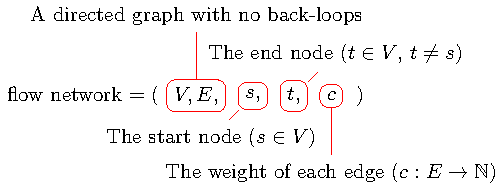
\includegraphics{equations/flow-network}
  \caption{}
  \label{fig:flow-network-definition}
\end{figure}

\textit{Back-loops} are a pair of edges that connect two nodes such that
$[(u,v),(v,u)]$

\begin{figure}[H]
  \centering
  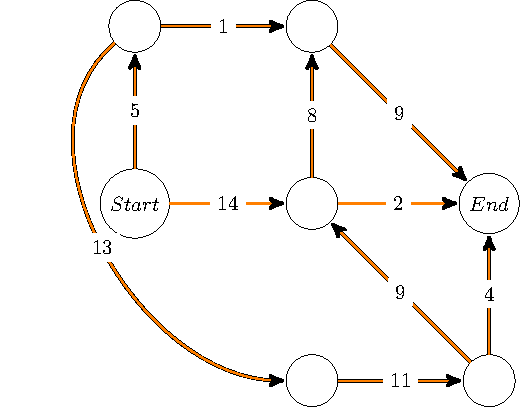
\includegraphics{diagrams/graph8}
  \caption{An example of a flow network. We assume that the start and edge 
    nodes have no incoming and outgoing edges respectively.}
  \label{fig:graph8}
\end{figure}

A \textbf{flow} over a flow network is a function $f : E \rightarrow
\mathbb{R^+}$ that has the following properties:

\begin{itemize}
  \item The net flow out of a node is zero.
  \item No edge exceeds its capacity ($f(u,v) \leq c(u,v)$).
  \item The \textit{value} of $f$ is the net flow out of the start node, or the
    net flow into the end node.
\end{itemize}

Our problem is that given a flow network $N$, we want to compute a flow for $N$
that has the maximum possible value (an optimal flow). If there is more than one
possible optimum flow, we don't mind which one is given.

In order to do this, we construct another graph (an \textit{auxiliary directed
graph}) from the one we're given. We construct the new graph by including all
the nodes, and following this rule for the edges; \textit{include an edge with
the value $c(u,v) - f(u,v)$ for all $u,v \in V$}.

This gives you the potential flow along each route. If an edge from $u$ to $v$
has a maximum capacity of $6$, but is carrying $2$, then in the auxiliary graph,
there should be an edge $(u,v)$ with a weight of $2$, and another from $(v,u)$
with a weight $4$ (since the flow can decrease by that much).

%TODO: Given example of creating an auxiliary graph

\subsubsection{The min-cut, max flow idea}

Remember, our end goal here is to get the maximum possible flow. The reason we
created an auxiliary graph in the first place, was because if there is a route
from the start node ($s$) to the end node ($t$) in it, then the flow is not
optimal.

Using this idea, we can make an algorithm to find the maximum flow:

\marginpar{I've made up some extra HashMap methods; increment and decrement. 
They assume that if the key isn't already associated with a value, the value 
was 0, and then they increment or decrement the value.}

\begin{lstlisting}[numbers=left,language=Java]
  Map<Edge, Integer> maximumFlow(List<Node> nodes, List<Edge> edges,
      Node start, Node end, Map<Edge, Integer> weight) {
    // Init the flow to all zeros
    Map<Edge, Integer> maxFlow = new HashMap<>();
    for (Edge e : edges) maxFlow.put(e, 0);
    // Iterate until we have a maximum flow
    while (true) {
      // Create the aux graph
      List<Edge> auxFlow = createAuxFlow(nodes, edges, flow, start, end);
      // Find the (possibly empty) path from the start to the end
      List<Edge> path = getPath(auxFlow, start, end);
      // If there is no path, then we're finished
      if (path.isEmpty()) break;
      else {
        for (Edge e : path) {
          // Increment each edge in the flow
          if (edges.contains(e)) maxFlow.increment(e);
          // If the edge isn't in the flow, decrement the edge going
          // the opposite way
          else maxFlow.decrement(e.reverse());
        }
      }
    }
    return maxFlow;
  }
\end{lstlisting}

If the flow network has integer capacities, then the optimal flow will have
integral values! This may be obvious in the above code, since the types are
integers, and we only ever increment or decrement.

We can find a path from any two nodes in linear time ($|V| + |E|$), as we do on
\texttt{Line 11}. If we define the constant $C$ to be the highest edge capacity,
then the maximum flow is $nC$, where $n$ is the number of nodes connected to the
start node, which could be $|V|$.

Therefore, the runtime of \texttt{maximumFlow} is $O(n(|V| + |E|)C)$

\subsubsection{Costs in flow networks}

What if we assigned every edge an associated cost that is charged per unit of
flow? We can add this to the definition of a flow network:

\begin{figure}[H]
  \centering
  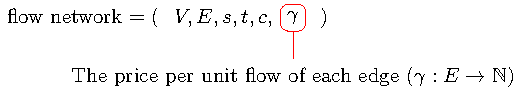
\includegraphics{equations/flow-network-costs}
  \label{fig:flow-network-definition-costs}
\end{figure}

%TODO: Add flow with costs

We can calculate the total cost of the flow to be:

\[
  \sum_{e \in E} f(e) \times \gamma(e)
\]

What if we want to find the maximum flow with the minimum cost? In fact, it is
possible to use the above \texttt{maximumFlow} algorithm to solve this, with
just a few small modifications; simply have the weight function $c$ take into
account $\gamma$:

\[
    c(e) = 
    \begin{cases}
        \gamma(e) & \text{if } (u,v) \text{is an edge in the aux graph, and in}
          ~E\\
        -\gamma(e) & \text{if } (u,v) \text{is an edge in the aux graph, and is
          not in}~E\\
    \end{cases}
\]

The only change we need to make on our flow finding algorithm is to find the
path from the start node to the end node using a minimal length:

\begin{lstlisting}[numbers=left,language=Java]
  Map<Edge, Integer> maximumFlow(List<Node> nodes, List<Edge> edges,
      Node start, Node end, Map<Edge, Integer> weight,
      Map<Edge, Integer> cost) {
    // Init the flow to all zeros
    Map<Edge, Integer> maxFlow = new HashMap<>();
    for (Edge e : edges) maxFlow.put(e, 0);
    // Iterate until we have a maximum flow
    while (true) {
      // Create the aux graph
      List<Edge> auxFlow = createAuxFlow(nodes, edges, flow, start, end);
      // Find the (possibly empty) path from the start to the end that has the
      // smallest cost
      List<Edge> path = getPath(auxFlow, start, end, cost);
      // If there is no path, then we're finished
      if (path.isEmpty()) break;
      else {
        for (Edge e : path) {
          // Increment each edge in the flow
          if (edges.contains(e)) maxFlow.increment(e);
          // If the edge isn't in the flow, decrement the edge going
          // the opposite way
          else maxFlow.decrement(e.reverse());
        }
      }
    }
    return maxFlow;
  }
\end{lstlisting}

This is the \textit{Busacker-Gowen algorithm}.

\subsection{Stable matching as a flow matching algorithm}

We can transform a matching problem into a flow matching problem as shown in
Figure~\ref{fig:matching-flow}.

\begin{figure}[H]
  \centering
  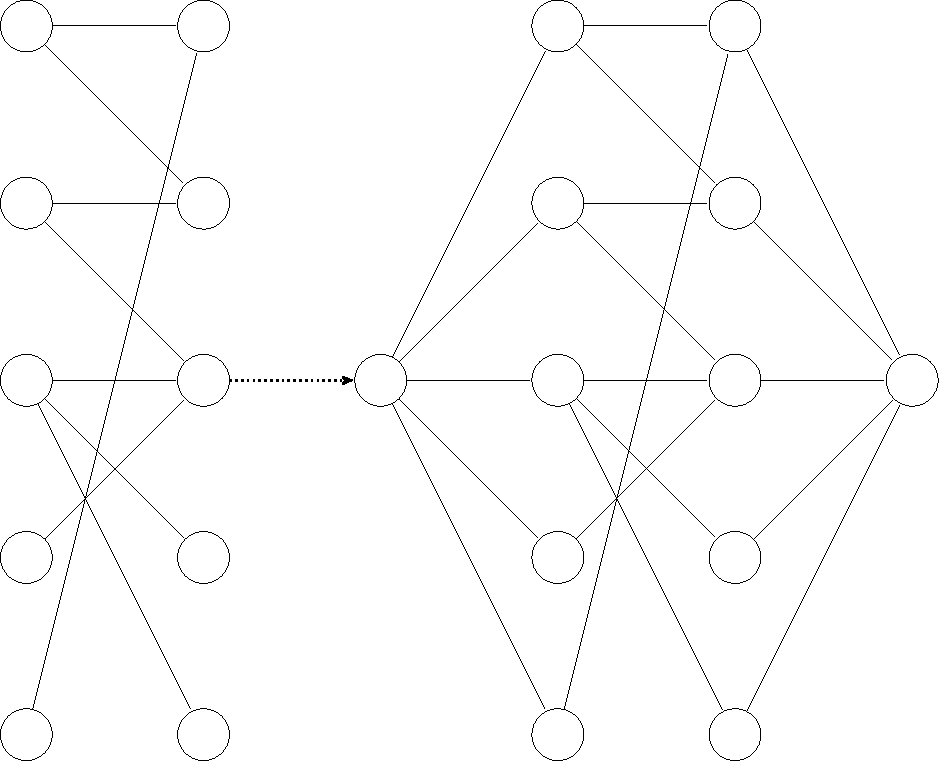
\includegraphics[width=0.6\textwidth]{diagrams/matching-flow}
  \caption{Here, a stable marriage problem (on the left, an edge indicates that
    both the boy and girl like each other) is mapped to a flow matching problem
    on the right.}
  \label{fig:matching-flow}
\end{figure}

We assume all the edge weights are $1$, and a perfect matching will be found iff
there is a flow from source to sink (the leftmost node to the rightmost node)
with a value $n$, where $n$ is the number of boys or girls. This runs on
$O(n(n+m))$ time!

\section{Turing Machines and Complexity Measures}

A Turing machine is a theoretical device that implements a model of computation.
It operates on a tape of infinite length, which is divided into cells, and can
read and write symbols from/to each cell when the \textit{head} of the machine
is positioned over the cell. The Turing machine also has internal state, which
is finite and determines what actions it takes (reading, writing, moving the
tape etc).

In this course, we will be thinking about multi-tape Turing machines. Here, the
there are many tapes, numbered $1 \dots K$. Tape $1$ is the input tape and tape
$K$ is the output tape. The tapes inbetween the input and output tapes are the
work tapes. Any algorithm can be expressed as a multi-tape Turing machine

\subsection{Formally defining a Turing Machine}

A TM (Turing Machine) can be define as a quintuple, as shown in
Figure~\ref{fig:tm-definition}.

\begin{figure}[H]
  \centering
  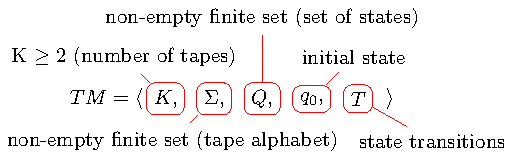
\includegraphics{equations/tm-definition}
  \caption{Part of a multi-tape Turing machine definition. We must also define
  the word \textit{symbol}, which is a mark occupying one cell on the tape. The
  alphabet that a symbol can be from is $\Sigma \cup \{
  \textrm{\textvisiblespace}, \vartriangleright\}$, where \textvisiblespace~is a
  blank cell, and $\vartriangleright$ is the start symbol (signifying the left
  edge of the tape).}
  \label{fig:tm-definition}
\end{figure}

Up to now, we've defined a TM that is perfectly formed\dots but does nothing. We
need to define how it moves between states in $Q$. To do that, we define a
transition, as in Figure~\ref{fig:tm-transition}.

\begin{figure}[H]
  \centering
  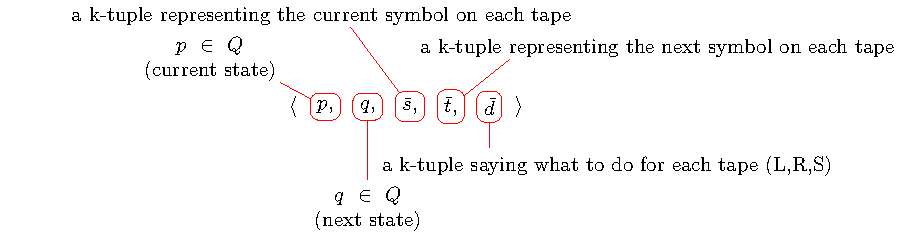
\includegraphics{equations/tm-transition}
  \caption{A transition of a Turing Machine}
  \label{fig:tm-transition}
\end{figure}

Informally, this transition applies only if the current state is $p$, and the
squares on the tapes confirm to $\bar{s}$, then set the new state to $q$ and
write the symbols from $\bar{t}$ to the tapes and move the heads as directed by
$\bar{d}$ (Left, Right or Stay).

Now we've nearly finished defining a multi-tape TM, the final points are:

\begin{itemize}
  \item Since the TM is deterministic, there can be \textit{at most} one 
    transition for every $(state,~\bar{current~symbols})$ tuple.
  \item The tape never moves left $\vartriangleright$.
  \item Tape 1 is read only and tape $K$ is write only.
\end{itemize}

\subsubsection{Acceptance, computability and decidability}

We say that a TM $M$ \textit{accepts} an input $x$ if it halts on $x$. The
language \textit{recognised} my $M$ is the set of strings that is accepted by
$M$.

\marginpar{Remember, when we say `Turing Machine', we could mean either a 
deterministic TM or a non-deterministic one (unless we explicitly said which one
we meant of course!).}

If a language is recognised by a Turing Machine $M$, then there is also a 
deterministic Turing Machine $M'$ that will recognise the same language. 

A language is \textit{computable} (aka decidable), if there is a (deterministic)
TM that will accept every string in the language, and reject every string not in
the language.

Up to now, our definitions of recognisable and computable are pretty similar (if
not the same). The difference is, that if an input string \textbf{isn't} in a
computable language, then the TM will halt (and output `no'), whereas if the
input string isn't in a recognisable language, then the TM \textit{may} halt and
output `no', or it could just carry on computing for ever. All a Turing Machine
does with a recognisable language, is recognise if a string is in the language,
it makes no guarantees about string not in the language!

\subsubsection{The Universal Machine}

If you're that way inclined, you can find lots of cool things about Turing
Machines. Another such cool thing, is that every TM is a finite thing (it's just
a quintuple as shown in Figure~\ref{fig:tm-definition}), which means we can come
up with a way of encoding any Turing Machine into a string over the alphabet
$\Sigma$ and use it as input to another Turing Machine!

If we can do this, then we can construct a \textbf{Universal Machine} $U$. This
machine takes two `arguments', another TM $M$ (encoded of course) and some
arbitrary input $x$. If $M \downarrow x$, then $U$ finishes with $y$ on its
output tape. If $M \uparrow x$, then $U$ will never terminate. The input is
coded as $M;x$, where `;' is a separator between the Turing Machine we're
`simulating' and the input we'll give it.

\subsubsection{Nailing that TM definition}

If you want your Turing Machines better defined than Arnie's Biceps, then this
how you do it (alternately, read Chapter 3 of Sipser).

%TODO: Not sure about a configuration on slide 8 of lecture 7b. I emailed Ian.

A run of a TM is terminating if it is finite. If the input to a deterministic TM
$M$ is $x$, and the run is finite, we write $M \downarrow x$ otherwise, if the
run is infinite, we write $M \uparrow x$.

Let $M$ be a deterministic TM that knows the alphabet $\Sigma$, and its input be
$x \in \Sigma*$ (i.e. the input is zero or more symbols from the alphabet). If
$M \downarrow x$ then the output tape of $M$ will contain some string $y \in
\Sigma*$ once M has finished computing. The cool thing, is that we can treat $M$
like a function, lets call it $f_M$, that operates over $\Sigma* \rightarrow
\Sigma*$:

\[
  f_M(x) = \begin{cases}
       y & if M \downarrow x\\
       \text{undefined} & if M \uparrow x\\
     \end{cases}
\]

In this case, $M$ computes the function $f_M$.

\subsubsection{Enumerators}

Enumerators aren't in the course slides, but they do appear in the reading. Skip
this section if you're doing last minute cramming.

An Enumerator is a Turing Machine with an attached printer. Now, I know what
you're thinking; \textit{I'm a computer scientist, I hate printers. Why would
anybody combine a complicated enough idea like a TM with a printer?!}
Enumerators have an important theoretical use though, and don't require us to
install drivers like we do for printers, and they certainly don't need to work
over WiFi (so this section should be a piece of cake really).

The TM inside an enumerator is able to send a string to the printer whenever it
wants to print out a string. If the TM does not halt, then the printer may print
an infinite list of strings. The language that is \textit{enumerated} by the
enumerator, is the collection of strings that it eventually prints out. Since
there are no rules about repetitions or ordering in the output list of the
printer, you might want to think about the enumerated language as a set.

So, as I said before, enumerators \textit{are} useful. Namely a language is
Turing recognisable if and only if, there is some enumerator that enumerates it.

Its easy to show that a TM can recognise a language that is enumerated by an
enumerator, just build a TM that does this:

\begin{enumerate}
  \item We have an input word $w$
  \item Run the enumerator $E$:
  \begin{enumerate}
    \item Every time $E$ outputs a new string, compare it to the word $w$
    \item If they are equal, then accept the word.
  \end{enumerate}
\end{enumerate}

Note that there is the potential for this TM to run for an infinite length of
time, if the enumerator generates an infinite list, and $w$ is not in the
language it enumerates.

We can also make an enumerator enumerate any language that is recognised by a
Turing Machine $M$:

\begin{enumerate}
  \item Ignore any input
  \item For $i = 1$ to $i = \infty$
  \begin{enumerate}
    \item Run the TM $M$ for $i$ steps for all possible strings of length $i$ in
      the language ($\Sigma^i$)
    \item If any computations accept, then print out the corresponding string.
  \end{enumerate}
\end{enumerate}

This enumerator will never halt (since it loops infinitely many times over an
infinitely large set of input strings), but eventually, it will print out all of
the words in the language (even though there will be \textit{a lot} of
duplicates!).

\subsection{The Halting problem}

The Halting problem asks:

\begin{quote}
  Given a Turing Machine $M$ and a string for its input $x$, return:
  \begin{itemize}
    \item[] \textbf{Yes} if $M \downarrow x$ ($M$ decides $x$)
    \item[] \textbf{No} otherwise, where $M$ would compute forever
  \end{itemize}
\end{quote}

Turing managed to prove that there is no Turing Machine that will decide the
Halting problem. The proof is fairly simple, but it takes a while to get your
head around it when its written in a mathematical form. Luckily, I found a poem,
written in the style of \href{https://en.wikipedia.org/wiki/Dr._Seuss}{Dr.
Seuss}, that provides a better textual explanation than I ever could; see
Figure~\ref{fig:halting-poem}.

\begin{figure}[h]
\begin{minipage}{\textwidth}
  \newgeometry{top=2cm,bottom=2cm,left=1cm,right=3cm}
  \begin{mymulticols}
  \poemtitle{Scooping the Loop Snooper\newline{\small An elementary proof of the 
  undecidability of the halting problem}}
\settowidth{\versewidth}{And this program called Q wouldn't stay on the shelf;}
\begin{verse}[\versewidth]
  No program can say what another will do.\\
  Now, I won't just assert that, I'll prove it to you:\\
  I will prove that although you might work til you drop,\\
  you can't predict whether a program will stop.

  Imagine we have a procedure called P\\
  that will snoop in the source code of programs to see\\
  there aren't infinite loops that go round and around;\\
  and P prints the word “Fine!” if no looping is found.

  You feed in your code, and the input it needs,\\
  and then P takes them both and it studies and reads\\
  and computes whether things will all end as they should\\
  (as opposed to going loopy the way that they could).

  Well, the truth is that P cannot possibly be,\\
  because if you wrote it and gave it to me,\\
  I could use it to set up a logical bind\\
  that would shatter your reason and scramble your mind.

  Here's the trick I would use - and it's simple to do.\\
  I'd define a procedure - we'll name the thing Q -\\
  that would take any program and call P (of course!)\\
  to tell if it looped, by reading the source;

  And if so, Q would simply print “Loop!” and then stop;\\
  but if no, Q would go right back to the top, \\
  and start off again, looping endlessly back,\\
  til the universe dies and is frozen and black.

  And this program called Q wouldn't stay on the shelf;\\
  I would run it, and (fiendishly) feed it itself.\\
  What behaviour results when I do this with Q?\\
  When it reads its own source, just what will it do?

  If P warns of loops, Q will print “Loop!” and quit;\\
  yet P is supposed to speak truly of it.\\
  So if Q's going to quit, then P should say, “Fine!” -\\
  which will make Q go back to its very first line!

  No matter what P would have done, Q will scoop it:\\
  Q uses P's output to make P look stupid.\\
  If P gets things right then it lies in its tooth;\\
  and if it speaks falsely, it's telling the truth!

  I've created a paradox, neat as can be -\\
  and simply by using your putative P.\\
  When you assumed P you stepped into a snare;\\
  Your assumptions have led you right into my lair.

  So, how to escape from this logical mess?\\
  I don't have to tell you; I'm sure you can guess.\\
  By reductio, there cannot possibly be\\
  a procedure that acts like the mythical P.

  You can never discover mechanical means\\
  for predicting the acts of computing machines.\\
  It's something that cannot be done. So we users\\
  must find our own bugs; our computers are losers!
\end{verse}
\attrib{Geoffrey~K.~Pullum, Scooping the loop snooper: An elementary proof of
the undecidability of the halting problem. Mathematics Magazine 73.4 (October
2000), 319-320}
  \end{mymulticols}
  \restoregeometry
\end{minipage}
\caption{A poetic explanation of the Halting Problem.}
\label{fig:halting-poem}
\end{figure}

As nice as it is, I think it's unlikely that the poem would be accepted as an
answer in an exam, so we'd better learn the formal definition of the Halting
problem too.

Suppose we have a TM $P$ that can determine if another TM can halt. We're going
to make another TM $Q$ that is defined so:

\begin{enumerate}
  \item Duplicate the input $x$ TM we're given.
  \item Run $P$ on the duplicated input ($x;x$).
  \begin{itemize}
    \item[] $P(x;x) = Y$, then Loop 
    \item[] $P(x;x) = N$, then Halt
  \end{itemize}
\end{enumerate}

Now, if we give $Q$ the input $Q$, then the embedded $P$ will receive $(Q,Q)$,
meaning that if:

\begin{description}
  \item $Q \downarrow Q \implies Q \uparrow Q$
  \item $Q \uparrow Q \implies Q \downarrow Q$
\end{description}

% TODO: Find another explination of the halting problem

\subsection{Complexity}

You already know that there are two types of Turing Machine; deterministic and
non-deterministic TM's, but now its time to think about the resources that
Turing Machines consume. We don't think of TM resources as commodities such as
metal, electricity etc, since TM's are abstract, theoretical devices. Instead
the two commodities we're interested in with Turing Machines are \textbf{time}
and \textbf{space}.

If we have a TM $M$, and let $g : \mathbb{N} \rightarrow \mathbb{N}$. $M$ runs
in time $g$ if for any finite input $x$, $M$ takes at most $g(|x|)$ steps. We
say that $M$ runs in space $g$ if for any finite $x$, $M$ takes at most $g(|x|)$
squares on its tapes.

If you think about it, this is nearly a formal way of defining the Big-Oh
notation. One of the main problems with this, is that TM's might execute at
different speeds (maybe one has faster motors for its tape etc). This means that
the algorithms we're designing will have certain runtimes on certain machines.
In order to mitigate this, we like to define sets of functions for the Big-Oh
notation; $M$ runs in time $G$ if for some $g \in G$, $M$ runs in time $g$.

This means that the Big-Oh notation can ignore things like constants, and lets
us abstract away the details of Turing machines (like exactly how many
operations it takes to multiply two numbers).

In fact, possibly the simplest definition of complexity is to let $L$ be a
language, and $G$ be a set of functions from $\mathbb{N}$ to $\mathbb{N}$. $L$
is in \texttt{TIME/SPACE(G)} if there exists a deterministic TM that recognises
$L$ in time/space G.

Similarly, if we can find a non-deterministic TM to recognise $L$, then we say
that $L$ is in \texttt{NTIME/NSPACE{G}}.

\subsubsection{Complexity classes}

As you probably know, there are several different complexity classes, as shown
in Table~\ref{tbl:complex-classes}.

\marginpar{Note, you can't have $Time(log(n))$ since reading the input takes
$n$ time.}

\begin{table}[h]
  \begin{tabular}{l >{$}l<{$} l >{$}l<{$}}
    & & LogSpace & Space(log(n))\\
    PTime & Time(n) & PSpace & Space(n)\\
    ExpTime & Time(2^{n}) & ExpSpace & Space(2^{n})\\
    k-ExpTime & Time(2^{2^{\dots^2\}^{n} \leftarrow k~times}}) & 
      k-ExpSpace & Space(2^{2^{\dots^2\}^{n} \leftarrow k~times}})\\
  \end{tabular}
  \caption{The deterministic complexity classes}
  \label{tbl:complex-classes}
\end{table}

To get their non-deterministic counterparts, just stick an `N' on the front of
everything, as in Table~\ref{tbl:complex-classes-nondet}.

\begin{table}[h]
  \begin{tabular}{l >{$}l<{$} l >{$}l<{$}}
    & & NLogSpace & NSpace(log(n))\\
    NPTime & NTime(n) & NPSpace & NSpace(n)\\
    NExpTime & NTime(2^{n}) & NExpSpace & NSpace(2^{n})\\
    Nk-ExpTime & NTime(2^{2^{\dots^2\}^{n} \leftarrow k~times}}) & 
      Nk-ExpSpace & NSpace(2^{2^{\dots^2\}^{n} \leftarrow k~times}})\\
  \end{tabular}
  \caption{The deterministic complexity classes}
  \label{tbl:complex-classes-nondet}
\end{table}

Obviously, some complexity classes can fit inside each other. Here are some
examples:

\[
  PTime \subseteq ExpTime \subseteq 2-ExpTime \subseteq \dots
\]

\[
  LogSpace \subseteq PSpace \subseteq ExpSpace \subseteq \dots
\]

\[
  NPTime \subseteq NExpTime \subseteq N2-ExpTime \subseteq \dots
\]

We can also interleave the non-deterministic classes:

\[
  PTime \subseteq NPTime \subseteq ExpTime \subseteq NExpTime \subseteq \dots
\]

Finally, the $Co^*$ complexity classes are the ones that describe the
complementary languages to those described by the others. For example, if we can
decide a language $L$ over $\Sigma^*$ in \texttt{NPTime}, then we can decide
$\Sigma^* - L$ in \texttt{Co-NPTime}. We know that \texttt{Time(G) =
Co-Time(G)}, and the same for space, but not if \texttt{NPTime(G) = Co-NPTime}.
